\section{Data and methods}
\subsection{General workflow}
\justify
This chapter describes the usage of methods in this study.

\begin{itemize}
    \item Kyselytutkimuksen teko
    \item Kyselytutkimuksen toteuttaminen
    \item geoprosessointi ja visualisointien tuotto
    \item Kyselytutkimuksen tulostentutkimus
    \item lopussa upea flowchartti
\end{itemize}

\begin{figure}[H]
    \centering
    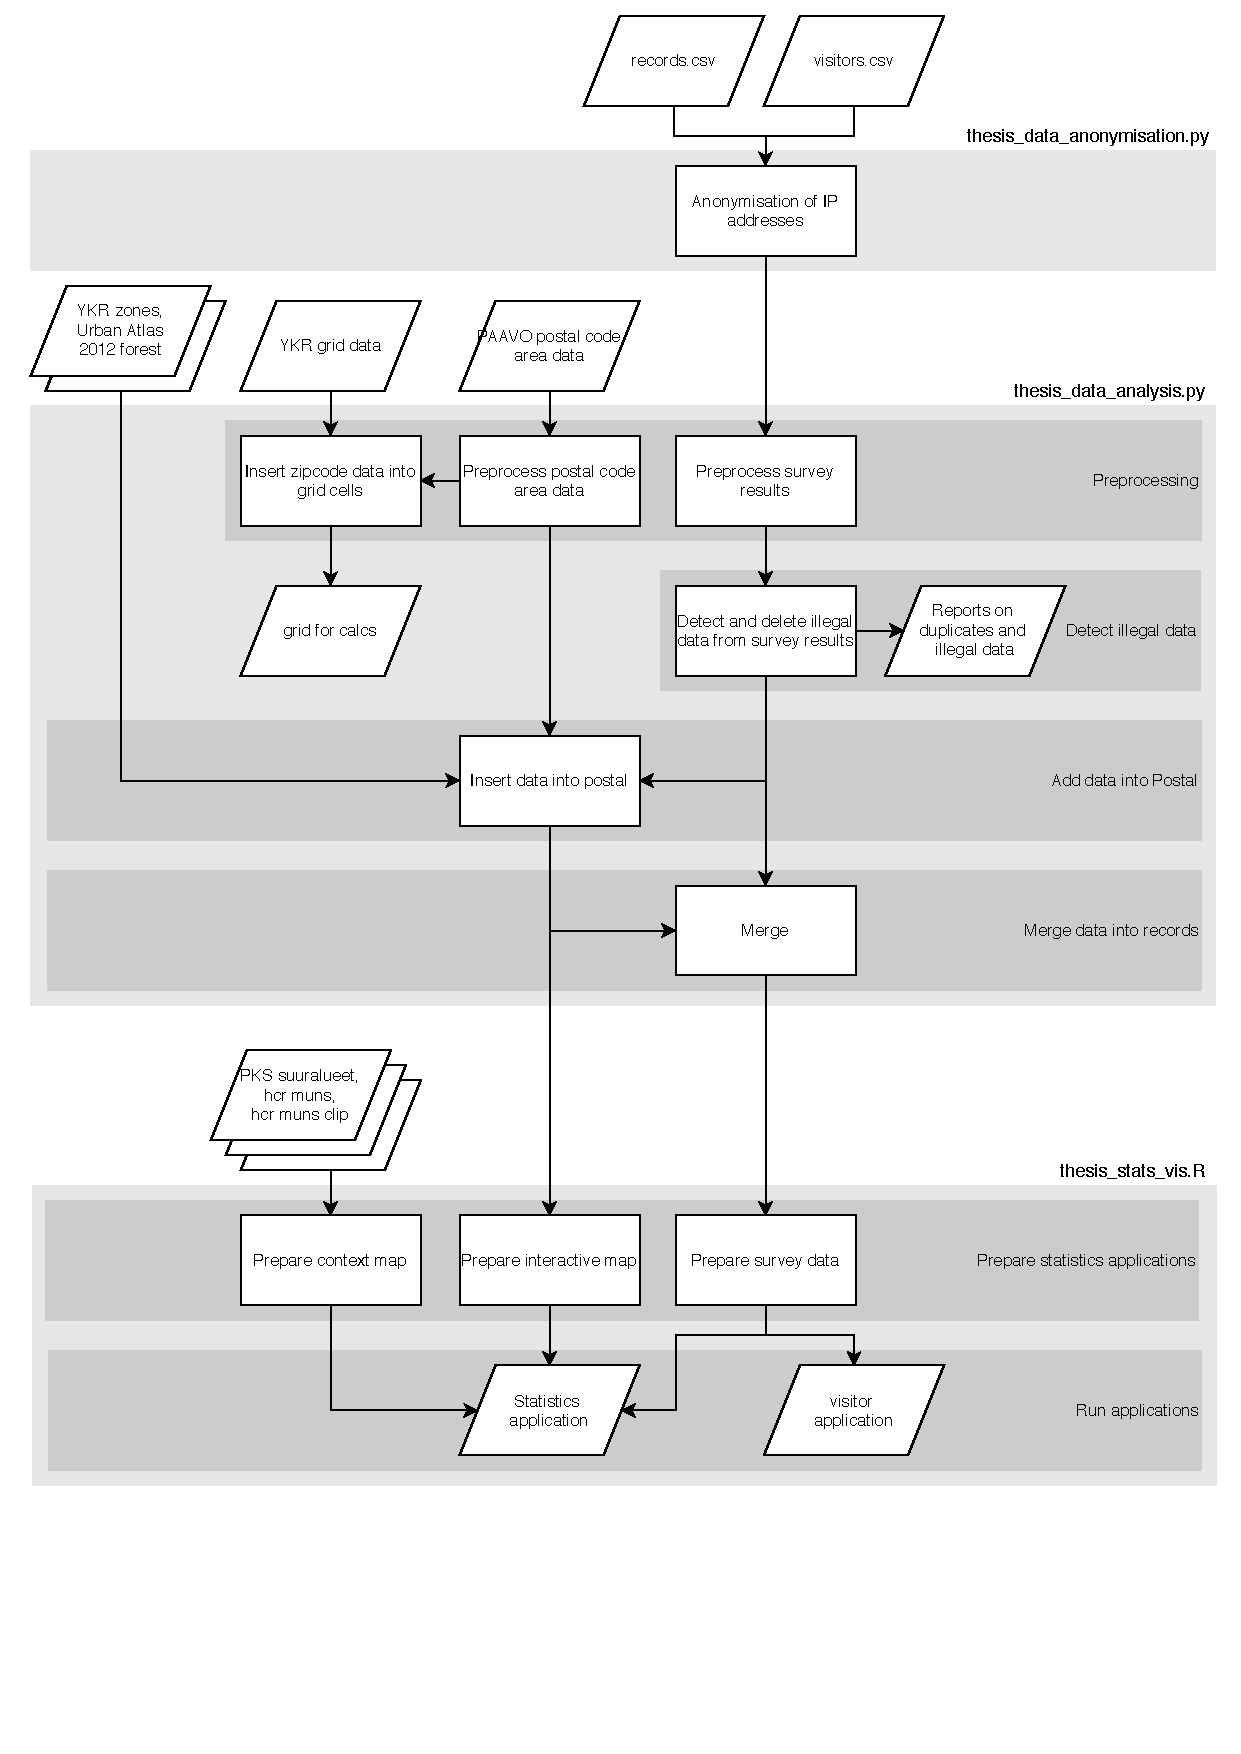
\includegraphics[trim=0.5cm 4.5cm 0.5cm 0.5cm,width=\columnwidth,scale=0.5]{thesis_workflow.pdf}
    \caption{General workflow in Python and R.} 
    \label{fig:gen_workflow}
\end{figure}

\subsection{Study area}
\justify
% https://www.hel.fi/hel2/Helsinginseutu/HS_tunnusluvut/liikennemaara_ja_autonomistus.pdf
% https://www.hsl.fi/sites/default/files/19_2016_auton_omistus_helsingin_seudulla.pdf
% https://www.hsl.fi/tutkimukset/muut-selvitykset
% http://pxnet2.stat.fi/PXWeb/pxweb/fi/StatFin/StatFin__lii__mkan/
The study area of this thesis is the Helsinki Capital Region. It comprises of municipalities of Helsinki, Espoo, Vantaa and Kauniainen. According to \textcolor{red}{LÄHDE}, the total population of the metropolitan area is 1.495 million. In practice the whole area amalgamates as one complete functional area with borders of the municipalities indistinguishable at the street level. The Helsinki Capital Region faces increasing pressure to manage its traffic because \textcolor{red}{LÄHDE}. Of these four municipalities Helsinki is the hub, and considered to contain the only inner city features of the municipalities (\textcolor{red}{syke-urbanareas}). Espoo, Vantaa and Kauniainen mostly consists of suburban areas with occasional industrial areas and large shopping complexes placed throughout the area. The Helsinki Capital Region is served with a high performance public transport system comprised of buses, train, subway, and tram in Helsinki. Recently, in 2017, the subway expanded from Helsinki to Espoo, triggering a new phase of quickly evolving cityscape in the surroundings of the new stations.

(\textcolor{red}{Insert map of the research area})

Despite the extensive service level of Helsinki Capital Region public transport, households especially in Espoo, Vantaa, and Kauniainen remain dependent on their personal vehicles (\textcolor{red}{LÄHDE}). 

\subsection{Data}
\justify

% hyphenrules: prevent hyphenation temporarily
\begin{hyphenrules}{nohyphenation}
    \begin{table}[H]
        \centering
        \caption{Data utilised in the thesis.} 
        \label{tab:useddata}
        % use \arraystretch to add whitespace between rows. \setlength\tabcolsep for columns
        \def\arraystretch{1.2} 
        \setlength\tabcolsep{1.2ex}
        % One unit here is ">{\raggedright\arraybackslash}p{4cm}". \raggedright prevents justification of text and conveniently allows flush right or flush left, which is not possible with column command p{4cm} alone.
        \begin{tabular}{ @{} >{\raggedright\arraybackslash}p{4cm} >{\raggedright\arraybackslash}p{4.5cm} >{\raggedright\arraybackslash}p{3.5cm} >{\raggedleft\arraybackslash}p{2.5cm} @{} }
            \toprule
            Data & Description & Producer & Citation \\
            \midrule
            Paavo -- Open data by postal code area & Helsinki Capital Region postal code areas & Statistics Finland & \cite{StatisticsFinland2019a} \\
            Urban Atlas 2012 & Land use and land cover data in vector format & European Environment Agency & \cite{EuropeanEnvironmentAgency2016} \\
            Zones of urban structure (Yhdyskuntarakenteen vyöhykkeet) 2017 & Delineation of urban areas based on the theory of urban fabrics & Finnish Environment Institute & \cite{Ristimaki2017} \\
            Helsinki Region-Travel Time Matrix 2018 & Travel time and distance information for routes between all YKR grid cell centroids in the Capital Region of Helsinki & Digital Geography Lab & \cite{Tenkanen2018} \\
            MetropAccess YKR grid & Statistical grid of 250 x 250 meters for monitoring urban structure, Helsinki Capital Region area & Statistics Finland & \cite{StatisticsFinland2020} \\
            \bottomrule
        \end{tabular}
    \end{table} 
\end{hyphenrules}

\subsection{Used software}
\justify

\begin{hyphenrules}{nohyphenation}
    \begin{table}[H]
        \centering
        \caption{Programming languages and \glspl{ide} utilised in the thesis.} 
        \label{tab:usedlangs}
        \def\arraystretch{1.3}
        \setlength\tabcolsep{1.2ex}
        \begin{tabular}{ @{} >{\raggedright\arraybackslash}p{3cm} >{\raggedright\arraybackslash}p{3.5cm} >{\raggedright\arraybackslash}p{2.5cm} >{\raggedright\arraybackslash}p{3cm} >{\raggedleft\arraybackslash}p{3cm} @{} }
            \toprule
            Programming language and \gls{ide} & Description & Purpose in thesis & Developer & Citation \\
            \midrule
            HTML, CSS, JavaScript (NetBeans 8.2.0) & Web technologies which enable interactive web sites & Research survey programming & WHATWG, W3C, ECMA\footnotemark, Apache Software Foundation & \cite{WHATWG2020}, \cite{W3C2020}, \cite{ECMA2019}, \cite{ApacheSoftwareFoundation2016} \\
            Python 3.7.6, Anaconda 2020.02 (Spyder 4.0.1) & Anaconda is a Python distribution for scientific computing & Survey data processing & Python Software Foundation, Anaconda, Inc., Spyder Project contributors & \cite{Python3Reference}, \cite{AnacondaInc.2020}, \cite{SpyderProjectContributors2020} \\
            R for Windows 3.6.3 (RStudio 1.2.5033) & Programming language environment for statistical computing & Survey data analysis and visualisation & R Core Team, RStudio, Inc. & \cite{RCoreTeam2020}, \cite{RStudioTeam2015} \\
            \bottomrule
        \end{tabular}
    \end{table} 
\end{hyphenrules}
% Normal footnotes in float objects do not work in Latex. Use \footnotemark and \footnotetext combo
\footnotetext{JavaScript is a trademark of Oracle Corporation in the United States. JavaScript is defined by European Computer Manufacturers Association (ECMA). JavaScript development is guided by an ECMA committee called TC39 which includes browser developers such as Google, Mozilla and Microsoft but also non-corporate members.}

\begin{hyphenrules}{nohyphenation}
    \begin{table}[H]
        \centering
        \caption{Essential software packages used in the thesis. The complete list is available at the script repositories in GitHub.} 
        \label{tab:usedsoft}
        \def\arraystretch{1.2}
        \setlength\tabcolsep{1.2ex}
        \begin{tabular}{ @{} >{\raggedright\arraybackslash}p{2.5cm} >{\raggedright\arraybackslash}p{2.5cm} >{\raggedright\arraybackslash}p{3.5cm} >{\raggedright\arraybackslash}p{3.5cm} >{\raggedleft\arraybackslash}p{3cm} @{} }
            \toprule
            Programming language & Software package & Purpose in thesis & Developer & Citation \\
            \midrule
            JavaScript & Leaflet 1.4.0 & Web mapping library for the research survey & Vladimir Agafonkin & \cite{Agafonkin2019} \\
            Python & pandas 1.0.1 & Data analysis and manipulation & Pandas contributors & \cite{McKinney2011a} \\
                & GeoPandas 0.5.0 & Geographic data operations & GeoPandas contributors & \cite{GeoPandasDevelopers2019} \\
                & Shapely 1.6.4.post1 & Geometric objects, predicates, and operations & Sean Gillies & \cite{Gillies2019} \\
                & rtree 0.8.3 & Spatial indexing & Sean Gillies, Howard Butler and contributors & \cite{Gillies2014} \\
            R & Shiny 1.4.0 & Web application framework for R & Shiny contributors & \cite{Chang2019} \\
                & ggplot2 3.3.0 & Data visualisation & ggplot2 contributors & \cite{Wickham2016} \\
                & ggiraph 0.7.0 & Interactive ggplot2 graphics & ggiraph contributors & \cite{Gohel2019} \\
                & dygraphs 1.1.1.6 & Interactive time series charting & dygraphs contributors & \cite{Vanderkam2018} \\
            \bottomrule
        \end{tabular}
    \end{table} 
\end{hyphenrules}

\subsection{Methods}
\justify

\subsubsection{Considering options for the survey}
\justify
(\textcolor{red}{Vois lisää kuvia näistä kokeiluista}) To collect the areal parking data, the study required an interactive survey which respondents could use to submit their parking habits in a spatial fashion. To attract a largest possible number of submissions, the survey also needed to be of modern design, easy to use and its purpose easy to understand. The survey would have to be clear-cut, effortless to internalise and short in length as to prevent users getting frustrated and leaving before submitting answers. Design-wise, the spatial resolution of the survey was in question. The particular concern was that in the case of insufficient amount of answers, what kind of area delineation would be at the same time detailed enough but also streamlined enough to realistically reach the good quality results? This chapter strives to describe the process that would lead to the implemented survey of the thesis to accentuate the challenges this kind of research entail.

Once the consideration into options to produce the survey for this study had started, it quickly became apparent that there were few alternatives available and even fewer free, sufficiently customisable alternatives. Out of the proprietary options, Maptionnaire by the Finnish company Mapita was considered. They offer tailored map survey products with discounts for students. In return for the fee a subscriber receives a time window in which to carry out their survey accompanied with tailored features and customer support -- all according to the price plan. This price was considered too steep for the thesis and Maptionnaire was passed on. 

Next Survey123 for ArcGIS was evaluated. An Esri operated service, Survey123 is used to create and analyse form based surveys (\cite{Esri}). It is included in the contract between University of Helsinki and Esri and thus was free to use for the study. One can design a survey at the Survey123 website and share it immediately to respondents. Alternatively, the service is available as a desktop client in the form of Survey123 Connect, where Survey123 offers a range of possibilities for customisation with its adherence to the XLSForm standard. XLSForm is a standard to make authoring forms in Excel easier. With the customisability of XLSForm users can design Survey123 surveys to the dot while employing the support for Excel style scripting for complex survey behaviour (figure~\ref{fig:survey123_xlsform}). Furthermore, Survey123 provides online tools for collaboration, analysis and data viewing with many options for exporting collected data. Some months were used to perfect the parking survey with Survey123. 

\begin{figure}[H]%
    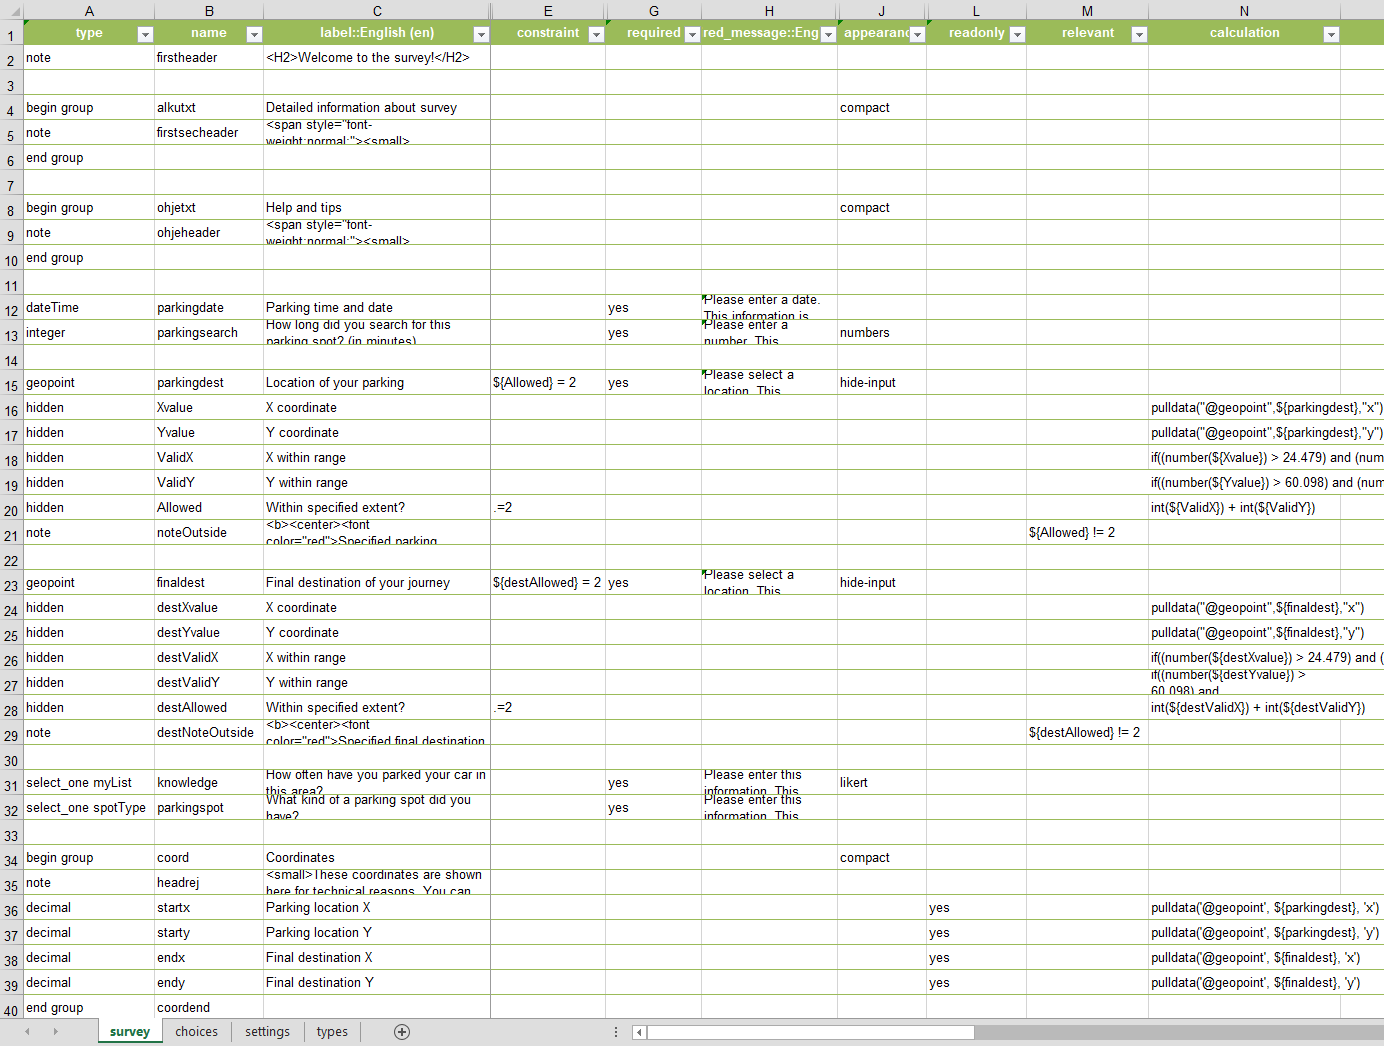
\includegraphics[width=\textwidth]{images/survey123_xlsform.png}
    \caption[Survey123 XLSForm view]{Survey123 XLSForm view in Microsoft Excel. Some parameter columns are hidden to provide a view to the essential inner workings of the Survey123 form.}%
    \label{fig:survey123_xlsform}%
\end{figure}

% \ref{}: tilde (~) indicates a non-breaking space
In January 2019 the parking survey developed with Survey123 was deployed to friends and family, with a large scale marketing push on social media platforms planned for later. At its core, this survey asked respondents for specific parking events in Helsinki Capital Region they had had (figure~\ref{fig:survey123}). Respondents would pick an exact location on a map view for the location of their parked car and separately on a second map view the location of their final destination. In addition, respondents would fill the date and time of this parking event, how long it took for them to find a parking spot, how often they had parked to that area, and what kind of a parking spot they had taken. Respondents were asked repeat this process as many times as they had the will to do so.

The Survey123 survey was designed to reach the same spatial resolution as Travel Time Matrix 2018 with the 250 x 250 meters YKR grid it utilises. Using exact coordinates of parkings and final destinations it would have been possible to allocate each event to possibly two different YKR grid cell codes, reaching excellent spatial resolution. As MetropAccess YKR grid contains 13 231 grid cells, there was not enough resources for this master's thesis research survey to accumulate events for every grid cell, or even for most grid cells. If the data gathering campaign would have ended with insufficient amount of parking events the backup plan was to employ an interpolation algorithm to generate approximate boundaries for the hypothetically varying parking times in Helsinki Capital Region. It was also considered that the exact coordinates of the parking events could be generalised to other boundaries, such as administrative areas like municipality subdivisions or postal code areas. 

% utilises package subfig
\begin{figure}[H]%
    \centering
    \subfloat[Survey introduction and the date and time for the parking event.]{{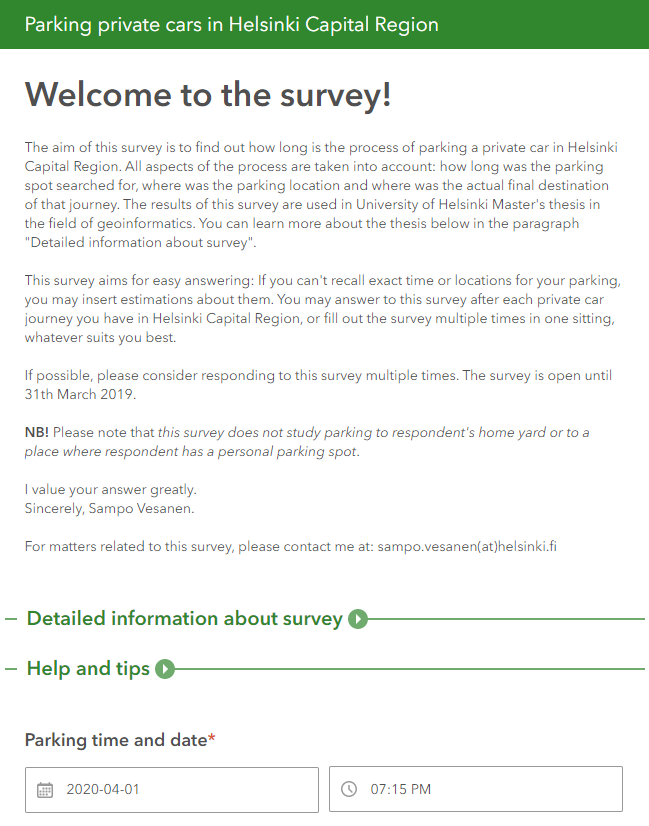
\includegraphics[width=5.5cm]{survey123_1.png} }}%
    \subfloat[Map panels for the parking location and the final destination.]{{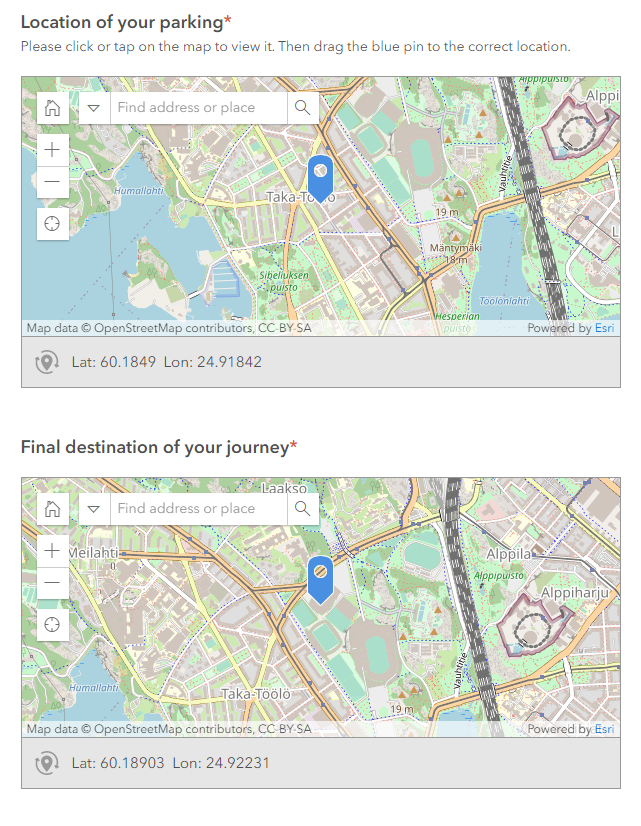
\includegraphics[width=5.5cm]{survey123_2.png} }}%
    \subfloat[Final questions of the survey.]{{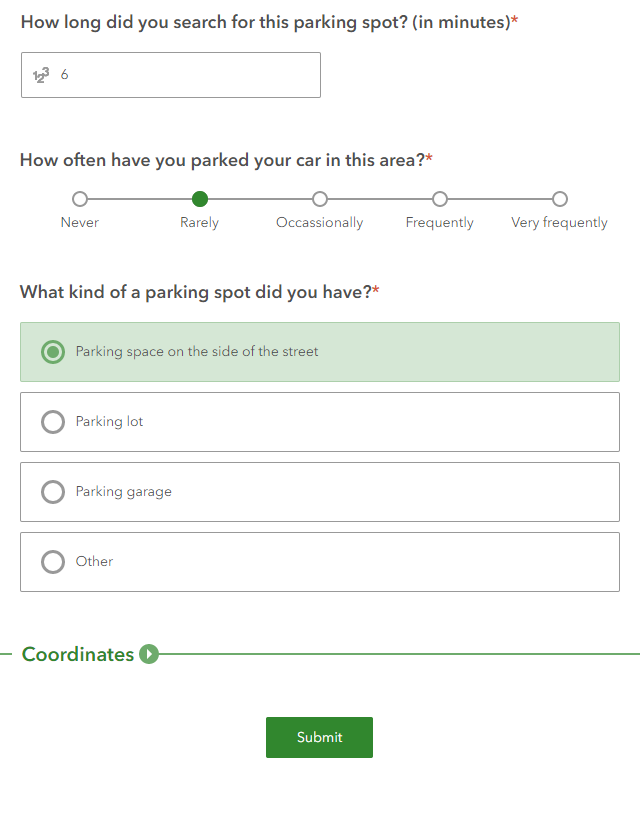
\includegraphics[width=5.5cm]{survey123_3.png} }}%
    \caption[The unused parking survey created with Survey123]{An example parking event entered into the unused parking research survey made with Survey123 Connect.}%
    \label{fig:survey123}%
\end{figure}

The survey was released even after Survey123 had proved itself unwieldly for the purposes of this research. The software was difficult to use because of an assortment of inconvenient design choices, unfinished functionality and a helping of bugs. It was not possible, for example, to have respondents enter multiple parking events at once in a full screen map view. They would have to reload the survey, something a majority of people would not do. Survey123 Connect version available at the time, version 3.1.126, did not allow customisation of the post-submission message and therefore it would not be possible to efficiently direct respondents back to the form. In addition, recording coordinates from two map views was only possible through a bypass. The coordinates of the final destination would have to be printed on the form (hence the section "Coordinates" on the form in figure~\ref{fig:survey123}) and then these second set of coordinates could be saved into the survey data table in string format. The technical limitations of Survey123 as a spatial survey was witnessed also in the fact that it was not possible to add custom polygons on top of the map views. It was therefore impossible to delineate the research area for the respondents and accurately detect attempts to add parking events outside of Helsinki Capital Region.

The functionality of the released form was not reliable on the most popular web browsers such as Google Chrome and Apple Safari. Survey123 supported multi-language strings but it proved problematic to ensure that the form would open in the system language of most respondents, Finnish. In addition to this, the field for entering the specific time of parking was restricted to the US preferred 12 hour clock -- a system Finnish nationals would frown upon in the survey. To make matters worse, at that time there was a long persisting bug in Survey123 which produced unexpected behaviour, in some cases, with the use of "constraint", the parameter that controls which entered values are deemed illegal and which are not (\cite{GeoNet-TheEsriCommunity2018}). If any type of constraint statement was added, the finalised form would always claim that the related question input was invalid. The parameter would have to be left empty and therefore it was not possible to automatically prevent insertion of parking events happening in the future and excessively long times for searching for parking, reducing the quality of the survey data and making the survey form more confusing for the respondent.

\begin{figure}[H]%
    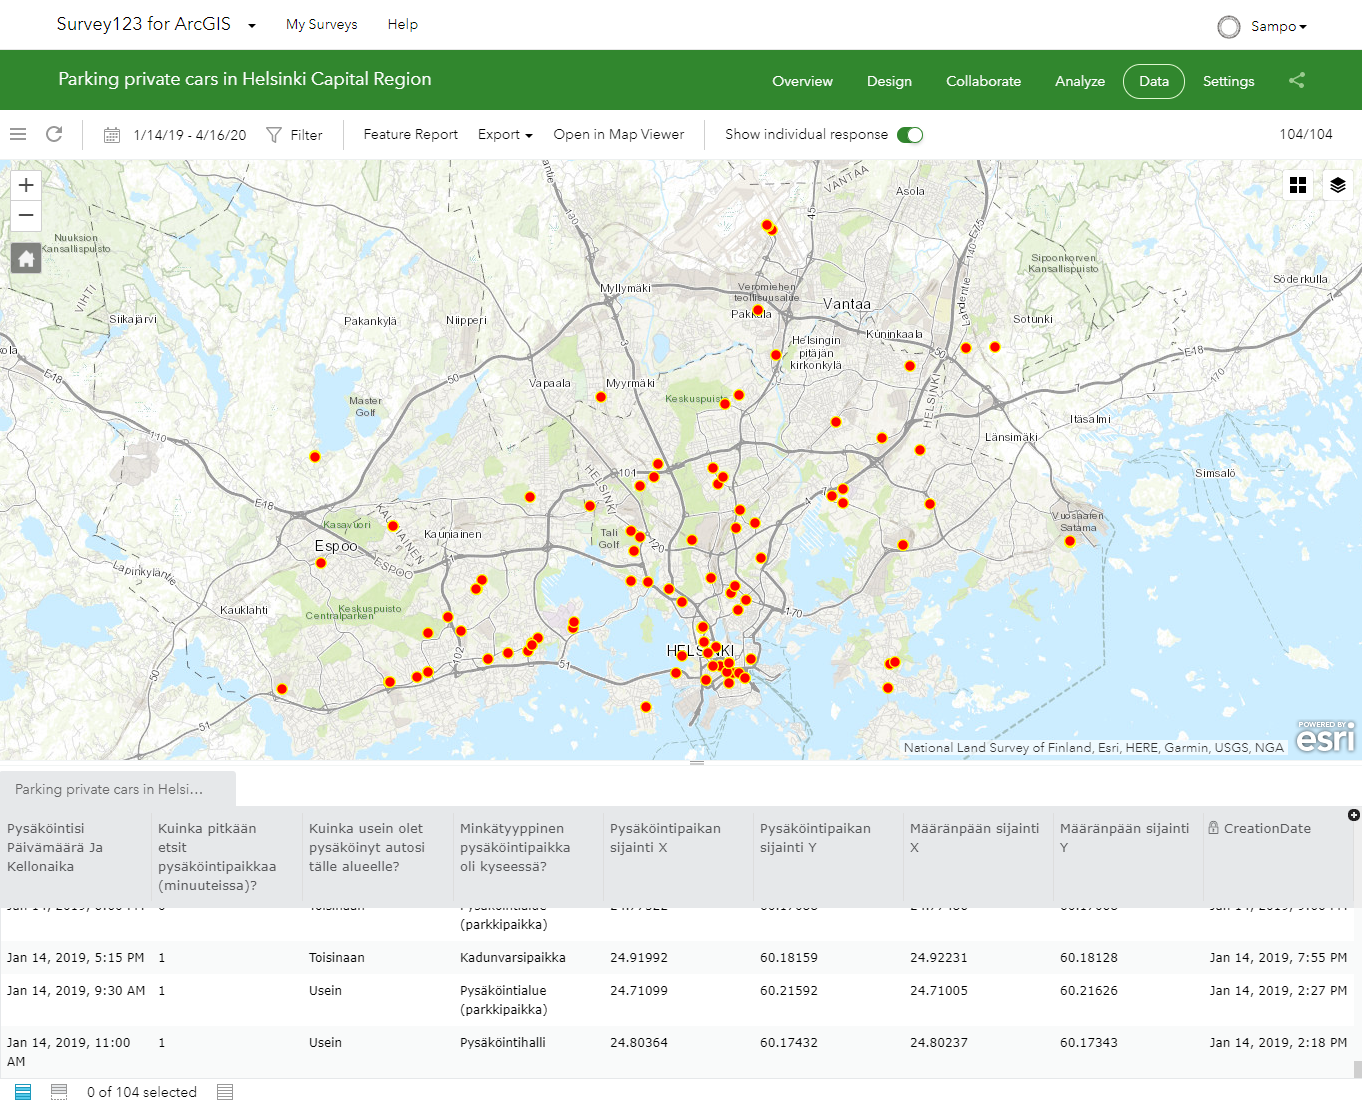
\includegraphics[width=\textwidth]{images/survey123_dataview.png}
    \caption[Survey123 data tab]{Survey123 for ArcGIS, with open "data" tab. The research survey made with Survey123 received in total 104 parking events. The red dots are the final destinations of each parking event.}%
    \label{fig:survey123_dataview}%
\end{figure}

Despite the many technical incertainties of Survey123, the survey gathered more than one hundred parking events in one month (figure~\ref{fig:survey123_dataview}). This amount was achieved for the most part without advertising. Soon after the publication of the Survey123 form it was decided, however, that the required spatial resolution for this research would need to be lower than exact points in an attempt to gather more responses from the entire research area. An additional deciding factor was the fact that with Survey123 respondents could not send multiple parking events with one survey session, making the form unwieldy and outdated in its rigid structured format. It was argued that a more general scale would still be accurate enough to provide good data and a more generalised scale would make the survey easier to answer to and a more pleasant experience for the respondent. Postal code areas were deemed an acceptable compromise in spatial accuracy.

After careful consideration it was decided that the survey for this thesis would have to be programmed from the ground up.

\subsubsection{Programming the parking survey}
\justify
To achieve maximum transparency and repeatability for this research, in addition to freedom in survey content and appearance, a survey web application was programmed from the ground up utilising HTML, JavaScript and PHP. The survey and its supporting infrastructure was installed on a virtual machine in CSC's -- the state owned ICT solutions company -- Taito supercluster. CSC offers virtual machines in several different hardware configurations, or flavors. The virtual machine flavor picked for this survey was \textit{standard.medium}, a flavor with 3.9 \gls{GB} \gls{RAM}, three virtual \gls{CPU}s and 80 GB of disk space. Running on the Linux distribution Ubuntu version 16.04, the backbone of the survey ecosystem was a LAMP stack, a software bundle which incorporates the Linux operating system, Apache web server software, \gls{mysql} relational database management system and the PHP programming language environment for server-side scripting. The public component of the survey is the front-end, the only component of the survey system a respondent would interact with (figure~\ref{fig:js_survey_welcome}). One may use additional software in a LAMP stack for extended functionality or can replace some of the components with a wide array of alternatives. This thesis utilises the components described in the table~\ref{tab:survey_components}.

\begin{hyphenrules}{nohyphenation}
    \begin{table}[H]
        \centering
        \def\arraystretch{1.2}
        \setlength\tabcolsep{1.2ex}
        \caption{Survey web application components} 
        \label{tab:survey_components}
        \begin{tabular}{ @{} >{\raggedright\arraybackslash}p{3cm} >{\raggedright\arraybackslash}p{3cm} >{\raggedright\arraybackslash}p{5.5cm} @{} }
            \toprule
            Component & Version & Description \\
            \midrule
            Ubuntu & 16.04.6 & Linux distribution, operating system for the virtual machine \\
            Apache HTTP Server & 2.4.18-2ubuntu3.9 & Web server software, manage website requests and responses \\
            MySQL & 5.7.25-0ubuntu0.16.04.2 & Relational database management system, survey database operations \\
            PHP & 7.0.33-0ubuntu0.16.04.1 & Programming language, used for server side scripting \\
            Parking survey front-end & 16.5.2019 & Survey visible to user, graphical user interface \\        
            \bottomrule
        \end{tabular}
    \end{table}
\end{hyphenrules}

Setting up the virtual machine for the use of the survey was a process of few stages. The LAMP stack was installed on the fresh virtual machine with the command \code{sudo apt install lamp-server\^}. \textcolor{red}{kuuluuko koodi graduun?} After the successful installation the MySQL tables were formed and relevant users created. The last step before a fully functioning web server was using root access to give the survey components permission to access relevant system directories. Please see the GitHub repository (\textcolor{blue}{\url{https://github.com/sampoves/parking-in-helsinki-region}}) for the full step-by-step install procedure used to set up the web server for this thesis.

\begin{figure}[H]%
    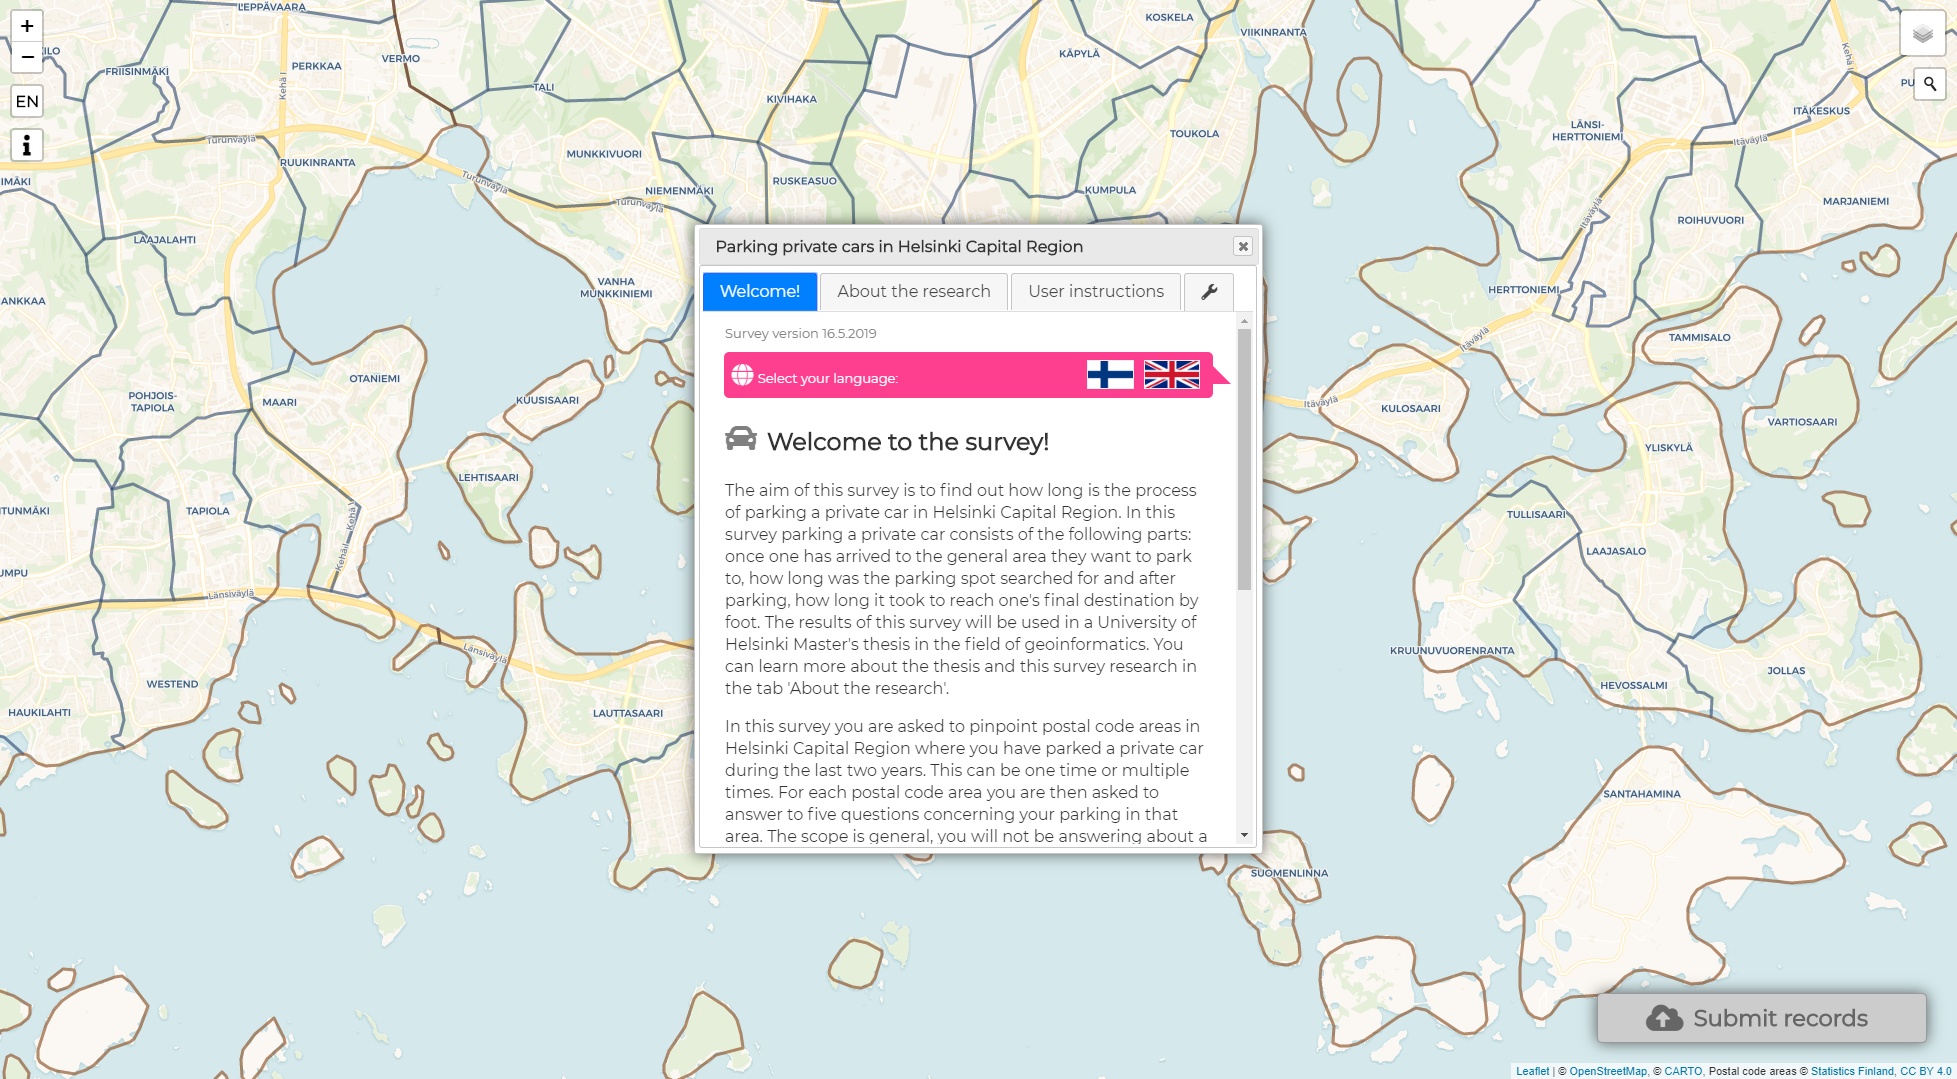
\includegraphics[width=\textwidth]{images/js_survey_welcome.png}
    \caption[Survey landing page]{This was the screen respondents would first see when arriving to the parking survey.}%
    \label{fig:js_survey_welcome}%
\end{figure}

The survey front-end was programmed in NetBeans \gls{ide} 8.2 in mostly JavaScript using an open-source mapping library Leaflet (software version 1.4.0) in January--May 2019. In the survey the respondent was presented with a map view of Helsinki Capital Region with its 167 postal code areas with the ability to drag the view, zoom in and out, search for places and addresses, choose the language between English and Finnish, and tweak various settings to their liking. In this setting, the respondent was asked to pick as many postal code areas as they could remember parking in in the last two years, and answer to five questions per postal code area (table~\ref{tab:js_survey_questions} and figure~\ref{fig:js_survey_questions}). In each question the respondent was asked to estimate their parking experience in that postal code area usually during the past two years. The last two years was chosen as the timeframe to allow respondents to comfortably recall parking events which happened during the subjective notion of "recent memory" while also forbidding the submission of out of date parking times. 

\textcolor{red}{lisää kappale, jossa selitän kysymysten sisällön auki?}

In the introduction to the survey it was explained to respondents that all answers were meant to be estimates as the survey was not about an exact time and place. To mitigate confusion and errors made by respondents a comprehensive help functionality and a location search tool were implemented in the parking survey. Once the respondent was finished with the survey, they would send their responses to the server. Respondents were welcomed to return to the survey to send additional data on any postal code areas they had missed the last time.

\begin{hyphenrules}{nohyphenation}
    \begin{table}[H]
        \centering
        \caption{Survey questions and question choices.} 
        \label{tab:js_survey_questions}
        \def\arraystretch{1.5}
        \setlength\tabcolsep{1.2ex}
        \begin{tabular}{ @{} >{\raggedright\arraybackslash}p{5.5cm} >{\raggedright\arraybackslash}p{5cm} >{\raggedleft\arraybackslash}p{2.5cm} @{} }
            \toprule
            Question & Question choices & Question type \\
            \midrule
            How long does it usually take for you to find a parking spot and park your car in this postal code area (in minutes)? & 0--99 & Field, selection within range \\
            How long does it usually take for you to walk from your parking spot to your destination in this postal code area (in minutes)? & 0--99 & Field, selection within range \\
            How familiar are you with this postal code area? & 1 -- Extremely familiar\linebreak2 -- Moderately familiar\linebreak3 -- Somewhat familiar\linebreak4 -- Slightly familiar\linebreak5 -- Not at all familiar & Radio button group, likert-type scale \\
            What kind of parking spot do you usually take in this postal code area? & 1 -- Parking space on the side of the street\linebreak2 -- Parking lot\linebreak3 -- Parking garage\linebreak4 -- Private or reserved spot\linebreak5 -- Other & Dropdown, selection \\
            At what time of the day do you usually park in this postal code area? & 1 -- Weekday, rush hour (07.00--09.00 and 15.00--17.00)\linebreak2 -- Weekday, other than rush hour\linebreak3 -- Weekend\linebreak4 -- None of the above, no usual time & Dropdown, selection \\
            \bottomrule
        \end{tabular}
    \end{table} 
\end{hyphenrules}

\begin{figure}[H]%
    \centering
    \subfloat[Survey questions in English.]{{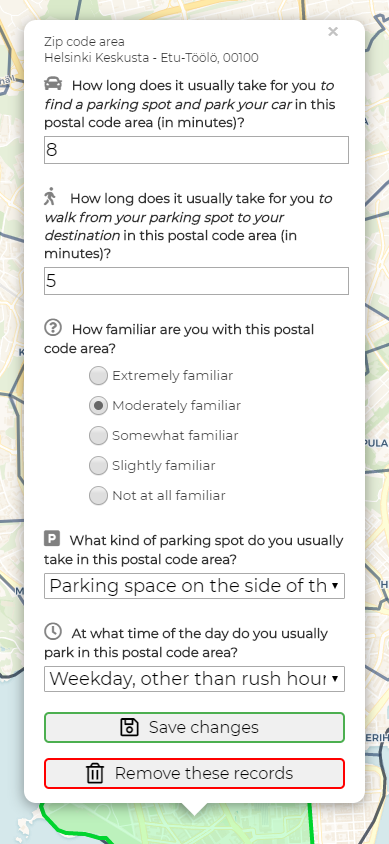
\includegraphics[width=6.25cm]{js_survey_en.png} }}%
    \qquad
    \subfloat[Survey questions in Finnish.]{{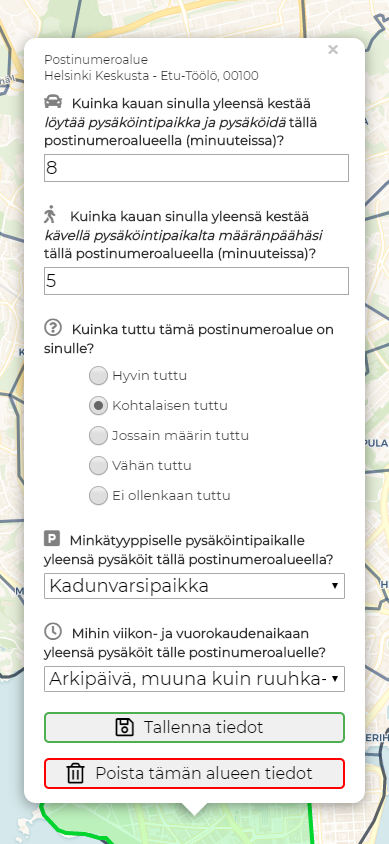
\includegraphics[width=6.25cm]{js_survey_fi.png} }}%
    \caption[Research survey questions in the web application]{For each postal code area of their choosing the respondent would answer to these five questions. The survey was made available in English and Finnish.}%
    \label{fig:js_survey_questions}%
\end{figure}

When data was received from the respondent, a script written in \gls{php} verified the data contents. This was an effort to prevent attacks on the web server running the study survey. Only specific variables of specific types were accepted from the front-end. Additionally, the \gls{php} verification made sure falsified or incomplete data would not be accepted into the database containing the verified results. If the server-side verification test failed in any way, the respondent was informed about it. 

In addition to the data verification, a PHP script tracked the IP addresses which accessed the survey web server. By using the survey, respondents agreed that their IP addresses were recorded for the use of this thesis solely to identify falsified or overlapping data and detect unique visits. All IP addresses were anonymised with a Python script and original sensitive data deleted. The anonymisation script is available for viewing at the survey repository at GitHub.

As a final survey component the server side contained two MySQL datatables, one for received data (Table~\ref{tab:mysql_records}) and another for survey web page hits (Table~\ref{tab:mysql_visitors}). In the table \textit{records}, the following data was recorded: time of sending (column name \code{timestamp}), IP address (\code{ip}), postal area code (\code{zipcode}), a value in the sequence 1--5 for the likert question (\code{likert}), a value in the sequence 1--5 for the question what type of parking spot was used (\code{parkspot}), an integer value for how long it usually took to park in this location (\code{parktime}), an integer value for how long it usually took to walk from parking place to one's destination (\code{walktime}), and a value in the sequence 1--4 for the question at what time of the day one usually parks in the location (\code{timeofday}). In the table \textit{records} it is notable that in the case an respondent sent the web server data for multiple postal code areas each of the postal code areas would take up their own row in the data table. Consequently, it was theoretically possible for one respondent to simultaneously submit 167 rows of data.

In the table \textit{visitors} the following data was recorded: IP address (\code{ip}), the timestamp of the first visit of this IP address (\code{ts\_first}), the timestamp of latest visit of this IP address (\code{ts\_latest}), and the count of visits (\code{count}). In this table an IP address is only stored once. On the first visit of an IP address the row for that IP address is created in the data table with \code{ts\_first} and \code{ts\_latest} being identical. On further visits of that IP address the original row is appended with updated information in the columns \code{ts\_latest} and \code{count}.

\begin{hyphenrules}{nohyphenation}
    \begin{table}[H]
        \centering
        \setlength\tabcolsep{1.2ex}
        \caption[Structure of MySQL table records]{The structure of the survey MySQL table \textit{records} fetched with the statement \code{DESCRIBE records;}} 
        \label{tab:mysql_records_str}
        \begin{tabular}{ @{} >{\raggedright\arraybackslash}p{2cm} >{\raggedright\arraybackslash}p{2cm} >{\raggedright\arraybackslash}p{1cm} >{\raggedright\arraybackslash}p{1cm} >{\raggedright\arraybackslash}p{1.5cm} >{\raggedleft\arraybackslash}p{4cm} @{} }
            \toprule
            Field & Type & Null & Key & Default & Extra \\
            \midrule
            id & int(11) & No & PRI & NULL & AUTO\_INCREMENT \\
            timestamp & varchar(19) & Yes & & NULL & \\
            ip & TEXT & Yes & & NULL & \\
            zipcode & varchar(5) & Yes & & NULL & \\
            likert & int(1) & Yes & & NULL & \\
            parkspot & int(1) & Yes & & NULL & \\
            parktime & int(2) & Yes & & NULL & \\
            walktime & int(2) & Yes & & NULL & \\
            timeofday & int(1) & Yes & & NULL & \\
            \bottomrule
        \end{tabular}
    \end{table} 
\end{hyphenrules}

\begin{hyphenrules}{nohyphenation}
    \begin{table}[H]
        \centering
        \setlength\tabcolsep{1.2ex}
        \caption[Structure of MySQL table visitors]{The structure of the survey MySQL table \textit{visitors} fetched with the statement \code{DESCRIBE visitors;}} 
        \label{tab:mysql_visitors_str}
        \begin{tabular}{ @{} >{\raggedright\arraybackslash}p{2cm} >{\raggedright\arraybackslash}p{2cm} >{\raggedright\arraybackslash}p{1cm} >{\raggedright\arraybackslash}p{1cm} >{\raggedright\arraybackslash}p{1.5cm} >{\raggedleft\arraybackslash}p{4cm} @{} }
            \toprule
            Field & Type & Null & Key & Default & Extra \\
            \midrule
            id & int(11) & No & PRI & NULL & AUTO\_INCREMENT \\
            ip & TEXT & Yes & & NULL & \\
            ts\_first & DATETIME & Yes & & NULL & \\
            ts\_latest & DATETIME & Yes & & NULL & \\
            count & int(11) & Yes & & NULL & \\        
            \bottomrule
        \end{tabular}
    \end{table} 
\end{hyphenrules}

The parking survey was released to the public in May 2019 and the active phase of collecting data continued until 30th June 2019. However, the survey remained open after the active period, receiving the last row of data in October 2019. The majority of the respondents were found through Facebook. Invitations to participate in the survey were sent to 112 city district and neighborhood groups with a theoretical reach of tens of thousands of people. Of the 112 posts, 63 were Helsinki centric groups, while 22 were from Espoo, 15 from Vantaa, and 12 from municipalities bordering Helsinki Capital Region. In addition to these city district and municipal groups invitation to participate was sent to two other Facebook groups, "Lisää kaupunki Helsinkiin", a group for city planning ethusiasts in Helsinki, and the GIS profession group "GIS-velhot". It is not possible to conclusively differentiate from which group or city survey data originated from. A clue about the survey's popularity in each city, however, may be gained from the table \textit{visitors} due to the fact that invitation posts were sent over multiple days to the groups in roughly the order Espoo--Helsinki--Vantaa--bordering municipalities--reminders to all groups. In addition to Facebook, an effort was also made to get faculty members of geosciences and geography and students of University of Helsinki to participate in the survey. A small amount of answers were collected with a tweet sent from the Twitter account of Digital Geography Lab. After the initial invitation to participate, reminders were sent to the largest Facebook groups one month after the original posts.

The source code for the survey described in this chapter and step-by-step information to set up an identical system is available at GitHub (\textcolor{blue}{\url{https://github.com/sampoves/parking-in-helsinki-region}}). As a side product, a variant of this survey was created where respondents pick precise points instead of areas. This point-based survey template is, too, available at GitHub (\textcolor{blue}{\url{https://github.com/sampoves/leaflet-map-survey-point}}).

% \scalebox to prevent table going too wide
\begin{hyphenrules}{nohyphenation}
    \begin{table}[H]
        \centering
        \setlength\tabcolsep{1pt}
        \caption[MySQL table records]{The data content of the survey MySQL table \textit{records}.} 
        \label{tab:mysql_records}
        \scalebox{0.92}
        {\begin{tabular}{ @{} >{\raggedright\arraybackslash}p{1.5cm} >{\raggedright\arraybackslash}p{4cm} >{\raggedright\arraybackslash}p{2.5cm} >{\raggedright\arraybackslash}p{2cm} >{\raggedright\arraybackslash}p{1.5cm} >{\raggedright\arraybackslash}p{1.5cm} >{\raggedright\arraybackslash}p{1.5cm} >{\raggedright\arraybackslash}p{1.5cm} >{\raggedleft\arraybackslash}p{1.5cm} @{} }
            \toprule
            id & timestamp & ip & zipcode & likert & parkspot & parktime & walktime & timeofday \\
            \midrule
            3245 & 2019-06-06 21:41:21 & wro4qo8hv4 & 00510 & 1 & 4 & 0 & 3 & 1 \\
            3246 & 2019-06-06 21:41:54 & aonm72lyx3 & 00520 & 2 & 1 & 10 & 5 & 1 \\
            3247 & 2019-06-06 21:46:19 & n1982i4i2v & 00100 & 1 & 1 & 20 & 4 & 1 \\
            3248 & 2019-06-06 21:46:22 & sbhfz0uvsl & 00210 & 1 & 1 & 5 & 3 & 3 \\
            3249 & 2019-06-06 21:46:22 & sbhfz0uvsl & 00220 & 2 & 2 & 5 & 5 & 2 \\        
            \bottomrule
        \end{tabular}}
    \end{table} 
\end{hyphenrules}

\begin{hyphenrules}{nohyphenation}
    \begin{table}[H]
        \centering
        \setlength\tabcolsep{1pt}
        \caption[MySQL table visitors]{The data content of the survey MySQL table \textit{visitors}.} 
        \label{tab:mysql_visitors}
        \begin{tabular}{ @{} >{\raggedright\arraybackslash}p{2cm} >{\raggedright\arraybackslash}p{3cm} >{\raggedright\arraybackslash}p{4cm} >{\raggedright\arraybackslash}p{4cm} >{\raggedleft\arraybackslash}p{1cm} @{} }
            \toprule
            id & ip & ts\_first & ts\_latest & count \\
            \midrule
            1780 & mvovd467a7 & 2019-05-26 15:25:23 & 2019-05-26 15:26:06 & 2 \\
            1781 & xgbgkkzxb3 & 2019-05-26 15:26:23 & 2019-05-26 15:26:23 & 1 \\
            1782 & c9qer4q99a & 2019-05-26 15:27:25 & 2019-05-26 15:27:25 & 1 \\
            1783 & cujhd0hng7 & 2019-05-26 15:27:29 & 2019-05-26 15:27:29 & 1 \\
            1784 & 3ja7gjtko6 & 2019-05-26 15:28:45 & 2019-05-26 15:29:20 & 2 \\        
            \bottomrule
        \end{tabular}
    \end{table} 
\end{hyphenrules}

\subsection{Processing survey data}
\label{sec:processdata} % labeling to enable hyperref to this chapter
\justify
%% pidä postal df mukana, muuten on sekavaa

%\begin{itemize}
%    \item anonymisation of ip addresses
%    \item Read in spatial data sources
%    \item Read in survey data
%    \item Prepare source data (convert formats, remove some irregular erroneous answers from dataset)
%    \item Prepare shape files (remove islands not reachable by car)
%    \item give grid cells zipcodes (ykr grid does not have those of-the-shelf. Develop method to assign all cells zipcodes, take into account water and grid cells which are outside of research area)
%    \item respondent behaviour (see how each user has answered)
%    \item detect illegal data (first detect duplicate answers, produce report. Then remove data where parktime and/or walktime is 60 or over)
%    \item Add data to geodataframes (add columns for ykr\_vyoh, ua-forest, answer count, parktime and walktime mean
%    \item show statistics to user
%    \item Set percentage of urban zones and forest in each zipcode area (choose one urban zone and forest amount (jenks breaks) for every zipcode)
%    \item add subdivisions to data (all answer row gets corresponding subdivision value)
%    \item EXPERIMENTAL utilise travel-time matrix 2018, make comparisons
%    \item EXPERIMENTAL somehow create my own TTM18, with updated values
%    \item export results to R
%\end{itemize}

The main objective of the thesis data processing was to merge the survey results with spatial data. Using a selection of open spatial data (table \ref{tab:useddata}), new explanatory spatial data would be available for analysis. This opened opportunities to compare the thesis survey data against that currently present in Helsinki Travel-time Matrix 2018. All data processing was carried out in Python 3.7.6, using Anaconda, a free and open-source Python distribution for scientific programming. Anaconda version 2020.02 included all essential packages for carrying out the script, except for GeoPandas 0.5.0, the package for geospatial data manipulation in Python. GeoPandas and its dependencies -- GDAL 2.4.1, Fiona 1.8.6, pyproj 2.1.3, rtree 0.8.3, and Shapely 1.6.4.post1 -- were manually installed through Python package installer pip.

As the first step in survey data processing, all IP addresses were anonymised. The anonymisation was carried out in such a way that the random identifiers for respondents matched in both textit{records} and textit{visitors}, preserving the possibility to associate survey responses with survey visits. 

\begin{figure}[H]%
    \centering
    \subfloat[Unedited PAAVO postal code areas for Helsinki Capital Region.]{{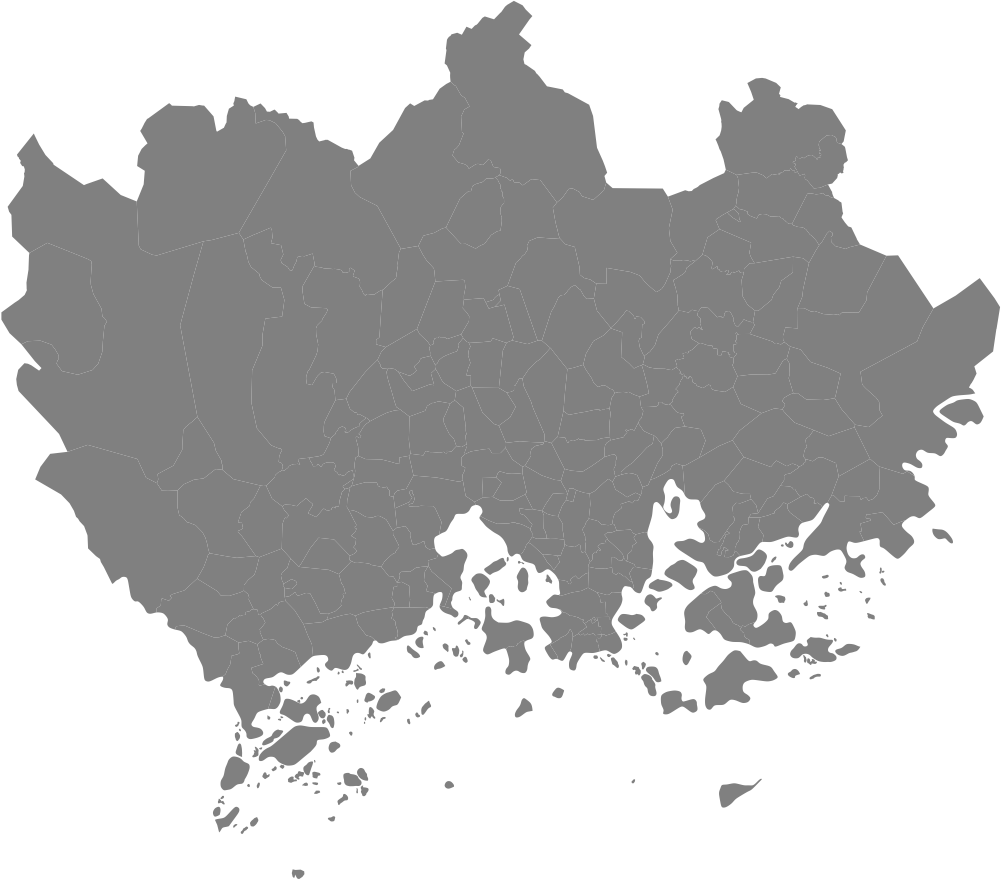
\includegraphics[width=8cm]{resarea_unedited.png} }}%
    \quad
    \subfloat[PAAVO postal code areas for Helsinki Capital Region, islands unreachable by car removed.]{{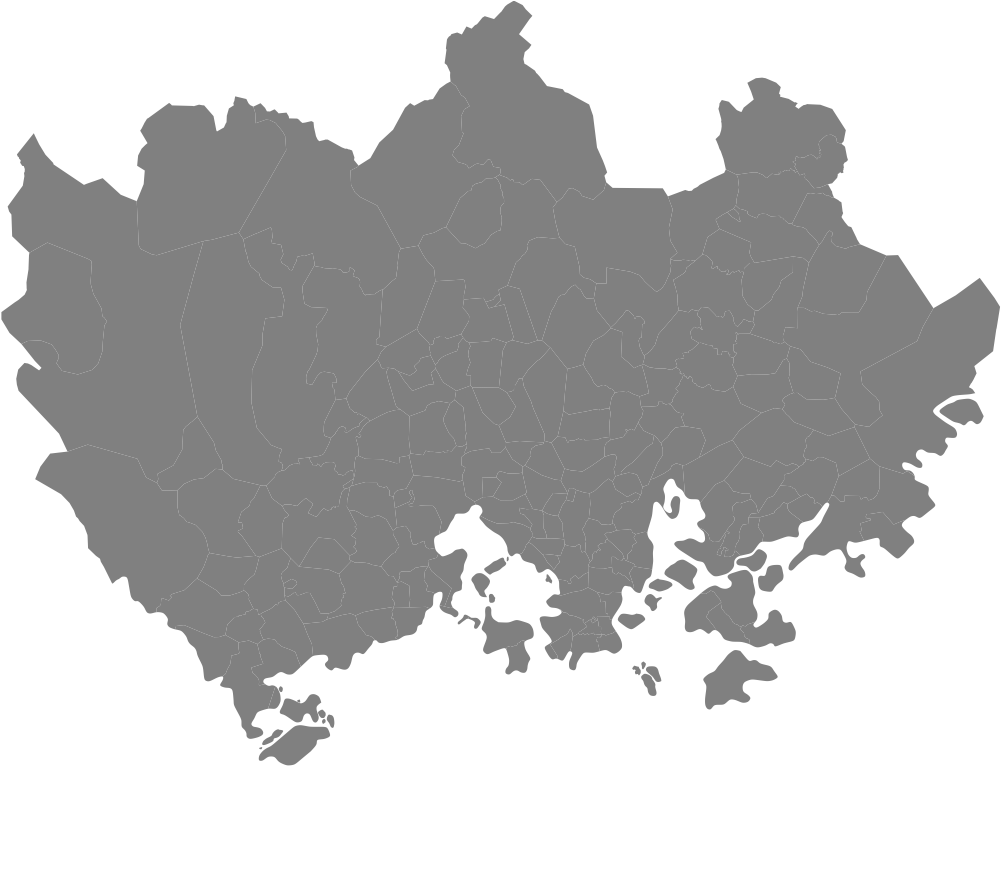
\includegraphics[width=8cm]{resarea_edited.png} }}%
    \caption[Process to remove islands not reachable by car]{Islands unreachable by car were removed from the postal code area data in the Python data processing.}%
    \label{fig:paavo_resarea}%
\end{figure}

The data processing proper started with loading the open spatial data presented in the table~\ref{tab:useddata} and selecting only those areas relevant to the research. Postal code areas were processed to only include areas reachable by car from the mainland in the research area (figure~\ref{fig:paavo_resarea}). Islands not reachable by car were approximated visually using Google Maps and were removed from the data.

Helsinki Travel-time Matrix 2018 and the survey data of this thesis operate in different spatial units. Travel-time Matrix 2018 uses the 250 x 250 meter Statistics Finland statistics grid and the basic spatial unit of the survey data is the postal code area. Using Python, postal codes were added to each grid cell with the logic that the largest area (\textcolor{red}{LISÄÄ KUVA}) assigns the postal code. PAAVO postal code areas are not present in all of the cells of YKR statistics grid and because of this some cells have a postal code of 99999 to denote missing data. In addition, the grid was merged with data which tells how much of a cell is contained in the research area and how large is the largest share which dictated the denotation of the current cell.

The data processing script created for this thesis contains detailed features to detect patterns in the survey data. To enable pattern recognition the records were purged of known false data, namely records and visits made by the author. In addition, one survey respondent reported that they had inserted erroneous data in the survey. These responses were identified and deleted.

A pandas DataFrame was created to make it easy to view the behaviour of each survey respondent. In addition to this feature, the data processing script writes a text file format report about respondents who have submitted multiple responses from the same postal code area. This report was then used to determine what to do about the duplicates.

It was decided that if parking time or walking time value was over 60 minutes that value would be deleted. This value is arbitrary and there is little reason (\textcolor{red}{voiko sanoa näin, hatusta heitetty?}) to believe that it would take anyone 60 minutes to reach their final destination from their place of parking. An hour of searching for parking plausible in the center of Helsinki. The data processing script deleted, additionally, the illegal IP address codes from visitors.

Next the additional spatial data was added to the survey data. Postal dataframe was added with answer count, parking time mean and walking time mean. Each postal code area also received seven columns to depict the share of classes in percentage. Using Urban Atlas 2012 data, all postal code areas were tested for forest percentage. Using a custom Jenks breaks function (by GitHub user Drewda, \textcolor{red}{miten citation?}) suitable class breaks were calculated to be used in records.

The dataframe records would be used as data in the analysis part of the thesis. Using the calculations made for dataframe postal, each row in records would receive, according to their postal code area, the most common urban structure type and the most common jenks break value. With data gathered from the Helsinki Capital Region web sites, using the postal code area in each response, the city subdivisions (Finnish "suuralue") were added to the dataframe records.

The source code for the data processing described in this chapter is available at GitHub (\textcolor{blue}{\url{https://github.com/sampoves/Msc-thesis-data-analysis}}).

\subsection{Conducting analyses}
% - Compare a few different travel time chains in Helsinki Capital Region. A few starting points and a few finishing points
% - All of the statistics stuff to detect the variation 
% - Tuuli was supposed to send me the exact numbers used for parking in Travel Time Matrix, did not do it yet

%\begin{itemize}
%    \item Prepare data to R compliant format
%    \item ShinyApp descriptive statistics
%    \item shinyapp histogram for parktime and walktime
%    \item shinyapp boxplot, show outliers
%    \item shinyapp barplot, show amounts
%    \item shinyapp levene test
%    \item shinyapp one-way anova
%    \item shinyapp map, nice to have, not at all important
%    \item visitor shinyapp, see the accumulation of visits and received records
%\end{itemize}
\justify
Once data processing in Python was completed, the survey data was carried over to R for its easy to access statistical analysis functionality (namely packages \textit{onewaytests} for ANOVA and Brown-Forsythe test, \textit{plotrix} for standard error, and \textit{moments} for quantiles) \textcolor{red}{citation}. To help viewing the large dataset of survey results, two Shiny applications were written, one for records and a second for visitors. The significance of this decision was twofold. Firstly, the interactive application allows switching variables on and off in the statistical tests in real time, making survey results analysis more efficient. Secondly, Shiny applications can be deployed to the Internet using the website shinyapps.io. This makes it effortless to display the results of this thesis in a visual way and uphold the thesis' mission of transparency as everyone can inspect the results and the tool themselves.

In the records tool users can view the survey data from multiple different angles. Users are given control which variables are active at any moment. The basis for the tool are the dropdown menus for continuous variables parktime and walktime and ordinal variables likert, parkspot, timeofday, ua\_forest, ykr\_zone, and subdiv. Any and all groups of values in the ordinal variables can be deactivated to better understand significance of each value. In addition to the selection of the continuous and ordinal variable, users can deactivate records based on their spatial location in research area subdivisions.

When the user has selected a continuous and an ordinal variable to compare, they are presented a thorough set of descriptive statistics with n, median, mean, standard deviation, standard error, confidence interval for lower and upper bound, minimum and maximum, 25 \% and 75 \% quantiles, skewness and kurtosis. For the continuous variables, a histogram is available to visualise the distribution of walktime and parktime. Distribution of ordinal variables likert, parkspot and timeofday can be compared against other ordinal variables in a barplot. To study quartiles, a boxplot is available. Imprortantly, users can test their selection of variables using the test of homogeneity of variables (Levene's test), analysis of variance (ANOVA), and the Brown-Forsythe test. Lastly, a context map of the research area is provided. The purpose of this map is to visualise which subdivisions are currently selected and which are deactivated.

Users can deactivate specific values from the currently selected ordinal variable at any time. In addition to this subdivisions of research area cities can be deactivated flexibly to better understand the spatial differences of the cities.

In visitors research tool users can view and examine events in the timeline of the survey research. In an interactive view cumulative charts are presented for received responses and survey page first visits. The charts reveal the effect of advertisement on actual records and survey traffic. Significance of different sources of responses can be viewed.

Scripts described in this chapter were written in RStudio 1.2.5033 using R for Windows 3.6.3. The source code for the data analysis and visualisation scripts are available at GitHub (\textcolor{blue}{\url{https://github.com/sampoves/Msc_thesis_data_analysis}}). The interactive analysis tools are available for testing on Shinyapps.io (\textcolor{blue}{\url{https://sampoves.shinyapps.io/records}} and  \textcolor{blue}{\url{https://sampoves.shinyapps.io/visitors}}). 